
\uc{Creazione conversazione libera}{conv_libera}
\begin{itemize}
    \item \textbf{Attori coinvolti}: Installatore;
    \item \textbf{Descrizione}: L’installatore desidera interrogare il sistema, quindi crea una nuova conversazione libera per richiedere le informazioni a lui necessarie tramite domande poste in linguaggio naturale;
    \item \textbf{Precondizioni}: L’installatore ha accesso all’interfaccia web del sistema;
    \item \textbf{Postcondizioni}: Il sistema crea una nuova conversazione libera a cui puó accedere l’installatore, dove potrà porre liberamente domande in linguaggio naturale al sistema;
    \item \textbf{Scenario principale}:
    \begin{enumerate}
    \item L’installatore accede all’interfaccia web di Vimar GENIALE;
    \item Richiede la creazione di una nuova conversazione in modalità libera;
    \item Il sistema esegue la creazione della nuova conversazione nella modalità desiderata dall’utente;
    \item  L’installatore accede alla nuova conversazione.
    \end{enumerate}
    \item \textbf{Estensioni}: UC 2 - Raggiungimento limite di conversazioni;
\end{itemize}
\begin{figure}[H]
\centering
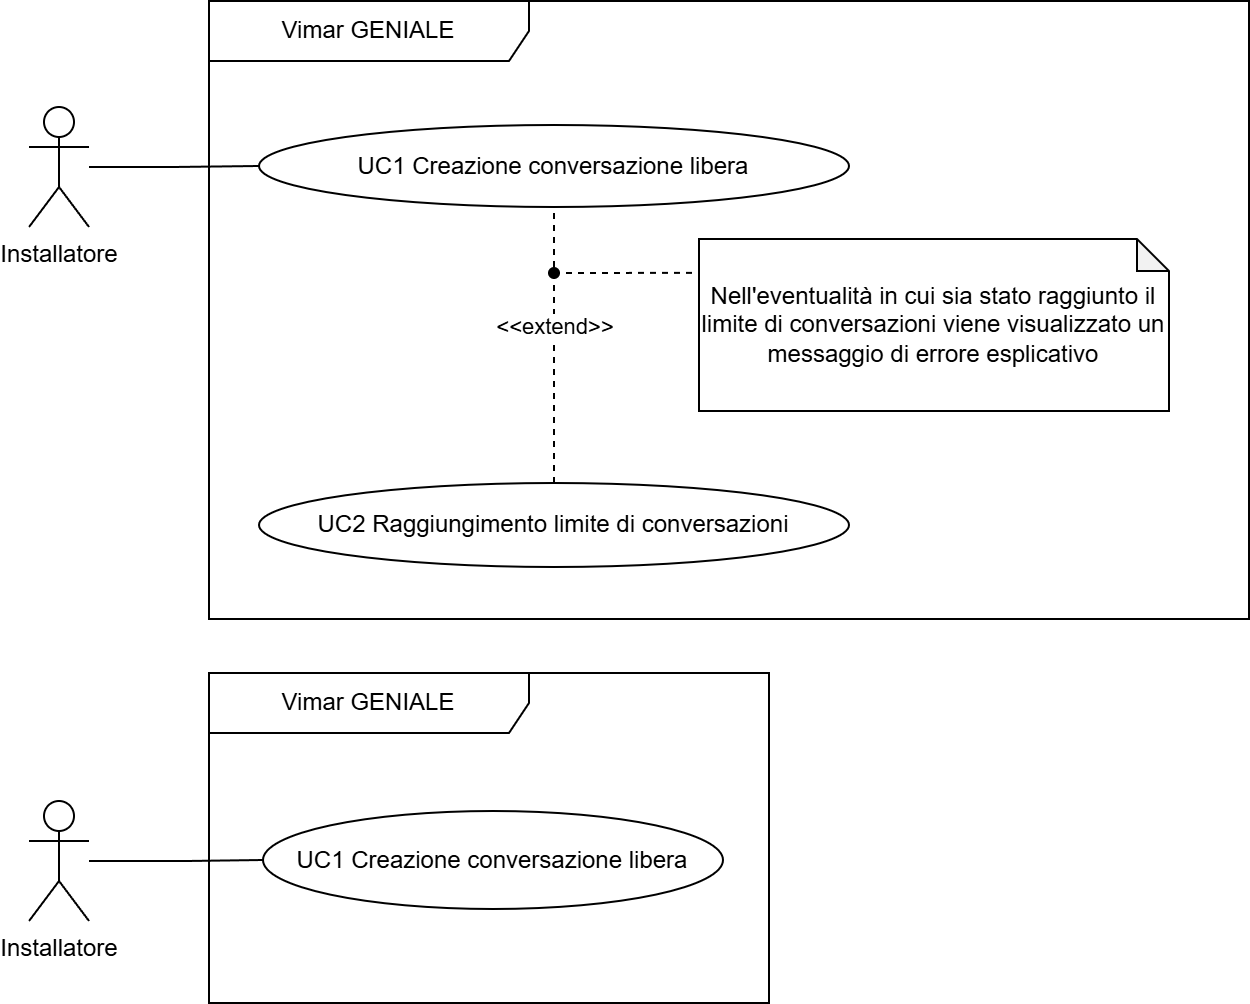
\includegraphics[width=0.8\textwidth]{contents/casi_duso/png/UC1.png}
\caption{UC1 - Creazione conversazione libera}
% \label{fig:UC1a}
\end{figure}

\uc{Raggiungimento limite di conversazioni}{limite_conv}
\begin{itemize}
    \item \textbf{Attori coinvolti}: Installatore;
    \item \textbf{Descrizione}: L’installatore desidera interrogare il sistema, ma quando prova a creare una nuova conversazione per richiedere le informazioni a lui necessarie, supera il limite massimo di conversazioni supportate;
    \item \textbf{Precondizioni}: 
        \begin{itemize}
            \item L’installatore ha accesso all’interfaccia web del sistema;
            \item Il numero di conversazioni memorizzate nel sistema supera il limite massimo supportato;
        \end{itemize}
    \item \textbf{Postcondizioni}:  Il sistema restituisce una risposta che indica il motivo per cui si è verificato l’errore;
    \item \textbf{Scenario principale}:
    \begin{enumerate}
    \item L’installatore accede all’interfaccia web di Vimar GENIALE;
    \item Richiede la creazione di una nuova conversazione, nonostante siano già esistenti un numero di conversazioni che raggiunge il limite;
    \item Il sistema elabora la richiesta e fornisce una risposta che spiega la causa dell'errore riscontrato;
    \item L’installatore visualizza le informazioni sull’errore che si è verificato.
    \end{enumerate}
\end{itemize}
\begin{figure}[H]
\centering
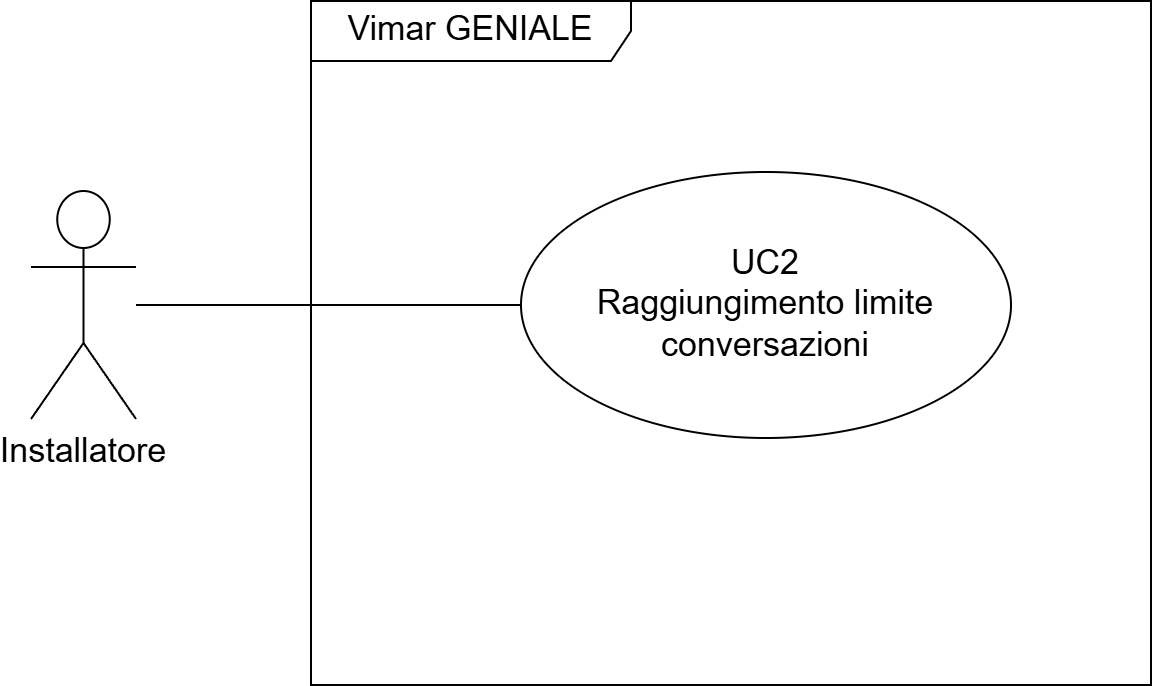
\includegraphics[width=0.8\textwidth]{contents/casi_duso/png/UC2.png}
\caption{UC2 - Raggiungimento limite di conversazioni}
\end{figure}


\uc{Salvataggio conversazione}{salvataggio_conv}
\begin{itemize}
    \item \textbf{Attori coinvolti}: Installatore;
    \item \textbf{Descrizione}: L’installatore, prima di chiudere l’applicativo, desidera salvare le conversazioni memorizzate attualmente all’interno del sistema, per poterle utilizzare nuovamente dal punto in cui ha concluso in precedenza alla prossima apertura dell’applicativo;
    \item \textbf{Precondizioni}: 
        \begin{itemize}
            \item L’installatore ha accesso all’interfaccia web del sistema;
            \item Sono presenti nel sistema un numero consentito di conversazioni;
        \end{itemize}
    \item \textbf{Postcondizioni}: Il sistema salva le conversazioni memorizzate attualmente all’interno del sistema;
    \item \textbf{Scenario principale}:
    \begin{enumerate}
    \item L’installatore accede all’interfaccia web di Vimar GENIALE;
    \item Richiede il salvataggio delle conversazioni esistenti al momento, prima di effettuare la chiusura dell’applicativo;
    \item Il sistema effettua il salvataggio e fornisce una risposta che conferma il completamento dell’operazione;
    \item L’installatore visualizza il messaggio di conferma dell’avvenuto salvataggio.
    \end{enumerate}
    \item \textbf{Estensioni}: UC 4 - Assenza di conversazioni durante il salvataggio
\end{itemize}
\begin{figure}[H]
\centering
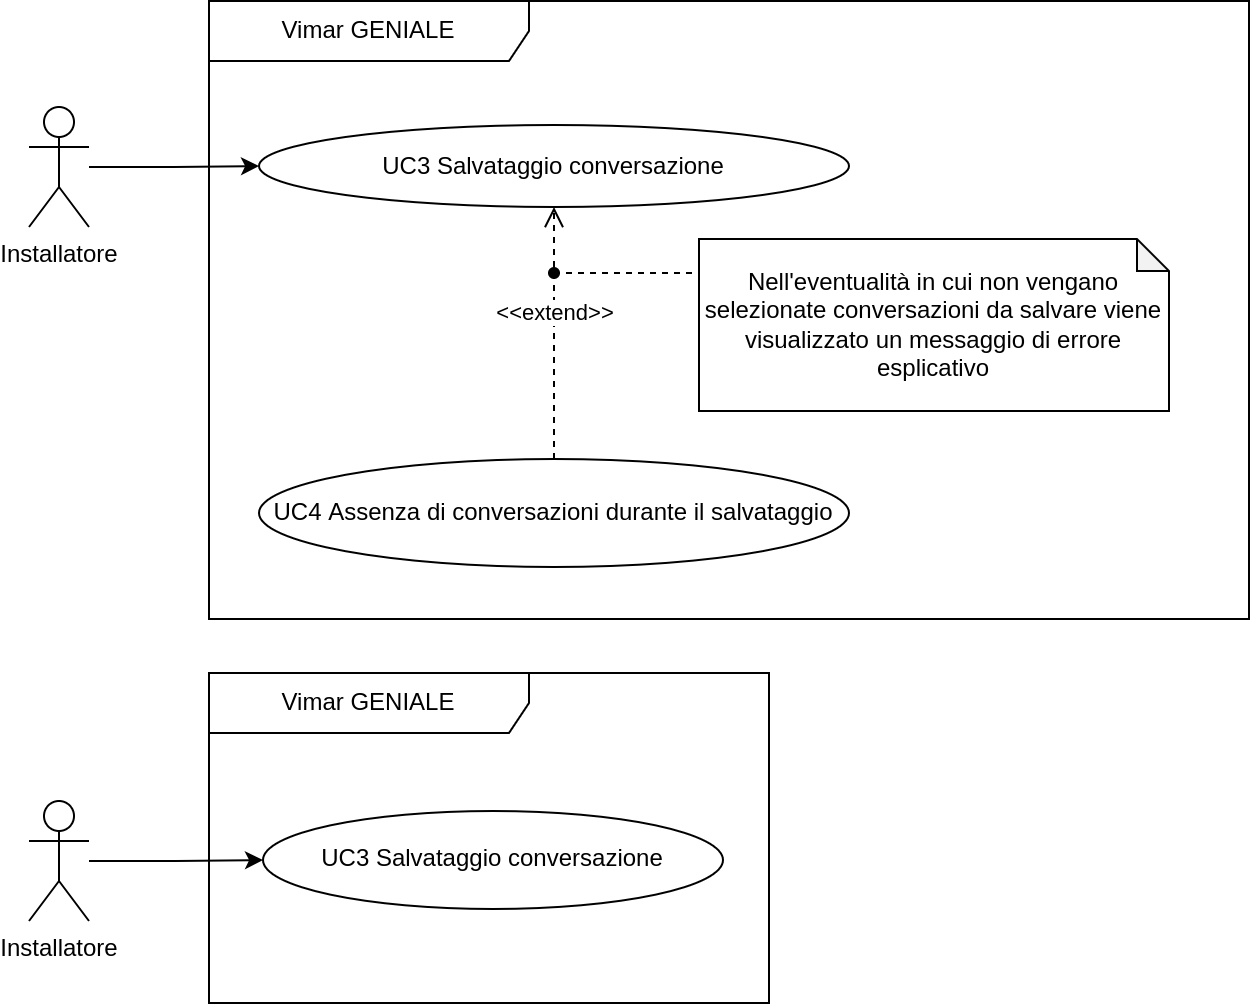
\includegraphics[width=0.8\textwidth]{contents/casi_duso/png/UC3.png}
\caption{UC3 - Salvataggio conversazione}
% \label{fig:UC1a}
\end{figure}

\uc{Assenza di conversazioni durante il salvataggio}{assenza_conv}
\begin{itemize}
    \item \textbf{Attori coinvolti}: Installatore;
    \item \textbf{Descrizione}: L’installatore tenta di salvare una o più conversazioni senza, però, che ce ne sia alcuna;
    \item \textbf{Precondizioni}: 
        \begin{itemize}
            \item L’installatore ha accesso all’interfaccia web del sistema;
            \item L'installatore crea una nuova conversazione libera e poi non fa nessuna domanda.
        \end{itemize}
    \item \textbf{Postcondizioni}: Il sistema restituisce una risposta che indica il motivo per cui si è verificato l’errore;
    \item \textbf{Scenario principale}:
    \begin{enumerate}
    \item L’installatore accede all’interfaccia web di Vimar GENIALE;
    \item L'installatore crea una nuova conversazione, ma non pone nessuna domanda.
    \item Richiede il salvataggio di una o più conversazioni;
    \item Il sistema elabora la richiesta e fornisce una risposta che spiega la causa dell'errore riscontrato;
    \item L’installatore visualizza le informazioni sull’errore che si è verificato.
    \end{enumerate}
\end{itemize}
\begin{figure}[H]
\centering
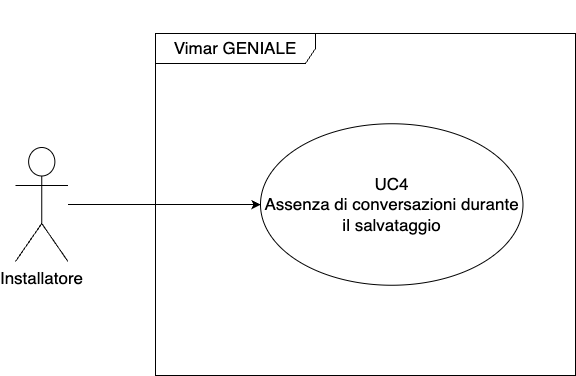
\includegraphics[width=0.8\textwidth]{contents/casi_duso/png/UC4.png}
\caption{UC4 - Assenza di conversazioni durante il salvataggio}
% \label{fig:UC1a}
\end{figure}


\uc{Cancellazione conversazione}{cancellazione_conv}
\begin{itemize}
    \item \textbf{Attori coinvolti}: Installatore;
    \item \textbf{Descrizione}: L’installatore desidera eliminare una conversazione esistente, in quanto non è ritenuta più necessaria al suo scopo;
    \item \textbf{Precondizioni}: 
        \begin{itemize}
            \item L’installatore ha accesso all’interfaccia web del sistema;
            \item L’installatore ha accesso ad una conversazione memorizzata nel sistema;
        \end{itemize}
    \item \textbf{Postcondizioni}: Il sistema elimina la conversazione non ritenuta più necessaria dall’installatore.
    \item \textbf{Scenario principale}:
    \begin{enumerate}
    \item L’installatore accede all’interfaccia web di Vimar GENIALE;
    \item Richiede l’eliminazione di una conversazione, in quanto ha raggiunto il suo scopo e non è più utile;
    \item Il sistema effettua l’eliminazione e fornisce una risposta che conferma il completamento dell’operazione;
    \item L’installatore visualizza il messaggio di conferma dell’avvenuta cancellazione.
    \end{enumerate}
\end{itemize}
\begin{figure}[H]
\centering
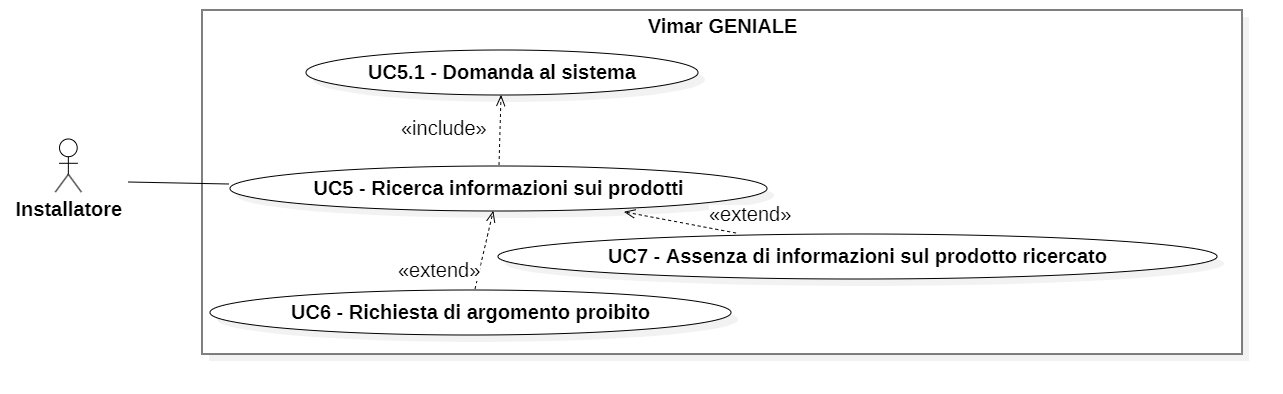
\includegraphics[width=0.8\textwidth]{contents/casi_duso/png/UC5.png}
\caption{UC5 - Cancellazione conversazione}
% \label{fig:UC1a}
\end{figure}


\uc{Ricerca informazioni sui prodotti con conversazione libera}{ricerca_info_prodotti}
\begin{itemize}
    \item \textbf{Attori coinvolti}: Installatore;
    \item \textbf{Descrizione}: L’installatore interroga il sistema per ottenere informazioni dettagliate su un prodotto specifico, come schemi elettrici, dati tecnici e manuali;
    \item \textbf{Precondizioni}: 
        \begin{itemize}
            \item L’installatore ha accesso all’interfaccia web del sistema;
            \item L’installatore ha accesso ad una conversazione memorizzabile nel sistema;
            \item Il prodotto richiesto è registrato nel sistema e le informazioni sono correttamente indicizzate.
        \end{itemize}
    \item \textbf{Postcondizioni}: Il sistema restituisce le informazioni richieste, incluse le descrizioni del prodotto, schemi elettrici e manuali di configurazione;
    \item \textbf{Scenario principale}:
    \begin{enumerate}
    \item L’installatore accede all’interfaccia web di Vimar GENIALE;
    \item Inserisce una domanda o una parola chiave relativa ad un prodotto specifico;
    \item Il sistema esegue la ricerca nel database le informazioni necessarie a fornire sufficiente contesto al LLM.
    \item LLM elabora la risposta;
    \item L’installatore visualizza la risposta.
    \end{enumerate}
    \item \textbf{Estensioni}: 
        \begin{itemize}
            \item UC 7 - Superamento limite caratteri del messaggio
            \item UC 8 - Assenza di informazioni sul prodotto ricercato
        \end{itemize}
\end{itemize}
\begin{figure}[H]
\centering
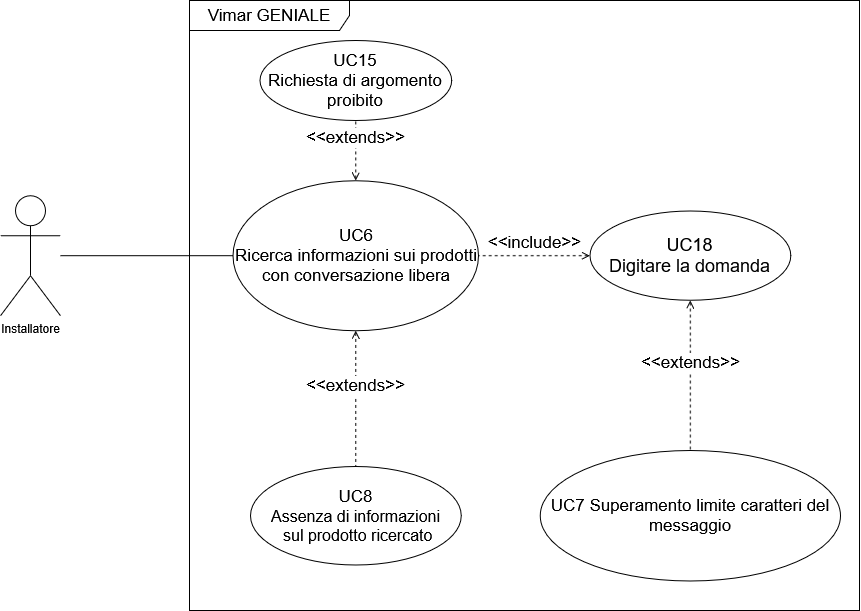
\includegraphics[width=0.8\textwidth]{contents/casi_duso/png/UC6.png}
\caption{UC6 - Ricerca informazioni sui prodotti con conversazione libera}
\end{figure}


\uc{Superamento limite caratteri del messaggio}{superamento_limite_caratteri}
\begin{itemize}
    \item \textbf{Attori coinvolti}: Installatore;
    \item \textbf{Descrizione}: L’installatore, quando interroga il sistema per ottenere informazioni, supera il limite di caratteri che possono essere utilizzati per effettuare la richiesta;
    \item \textbf{Precondizioni}: 
        \begin{itemize}
            \item L’installatore ha accesso all’interfaccia web del sistema;
            \item L’installatore ha accesso ad una conversazione memorizzabile nel sistema;
            \item La domanda posta supera il limite massimo di caratteri consentiti.
        \end{itemize}
    \item \textbf{Postcondizioni}: Il sistema restituisce una risposta che indica il motivo per cui si è verificato l’errore;
    \item \textbf{Scenario principale}:
    \begin{enumerate}
    \item L’installatore accede all’interfaccia web di Vimar GENIALE;
    \item Inserisce una domanda o una parola chiave relativa ad un prodotto specifico, superando il limite massimo consentito di caratteri;
    \item Il sistema elabora la richiesta e fornisce una risposta che spiega la causa dell'errore riscontrato;
    \item L’installatore visualizza le informazioni sull’errore che si è verificato.
    \end{enumerate}
\end{itemize}
\begin{figure}[H]
\centering
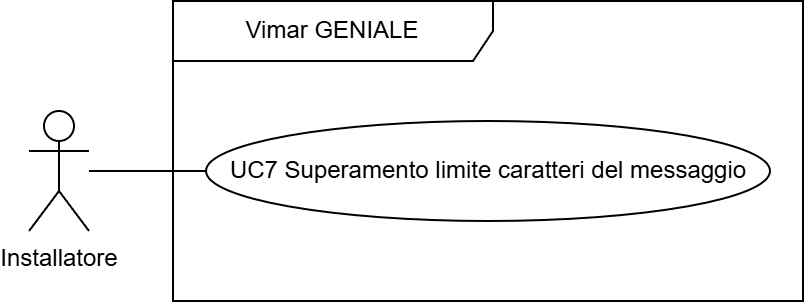
\includegraphics[width=0.8\textwidth]{contents/casi_duso/png/UC7.png}
\caption{UC7 - Superamento limite caratteri del messaggio}
% \label{fig:UC1a}
\end{figure}


\uc{Assenza di informazioni sul prodotto ricercato}{assenza_info_prodotto}
\begin{itemize}
    \item \textbf{Attori coinvolti}: Installatore;
    \item \textbf{Descrizione}: L’installatore interroga il sistema per ottenere informazioni dettagliate su un prodotto specifico, ma il sistema non è in grado di trovare nessuna informazione relativa ad esso;
    \item \textbf{Precondizioni}: 
        \begin{itemize}
            \item L’installatore ha accesso all’interfaccia web del sistema;
            \item L’installatore ha accesso ad una conversazione memorizzabile nel sistema;
            \item L’installatore pone una domanda al sistema;
            \item Il sistema non è in possesso di alcuna informazione relativa al prodotto ricercato.
        \end{itemize}
    \item \textbf{Postcondizioni}: Il sistema restituisce una risposta che indica il motivo per cui si è verificato l’errore;
    \item \textbf{Scenario principale}:
    \begin{enumerate}
    \item L’installatore accede all’interfaccia web di Vimar GENIALE;
    \item Inserisce una domanda o una parola chiave relativa ad un prodotto specifico;
    \item Il sistema elabora la richiesta e fornisce una risposta che spiega la causa dell'errore riscontrato;
    \item L’installatore visualizza le informazioni sull’errore che si è verificato.
    \end{enumerate}
\end{itemize}
\begin{figure}[H]
\centering
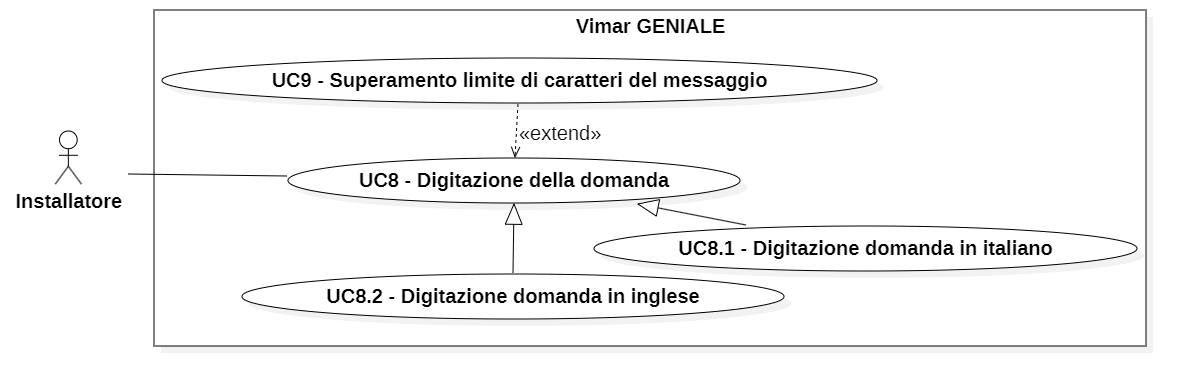
\includegraphics[width=0.8\textwidth]{contents/casi_duso/png/UC8.png}
\caption{UC8 - Assenza di informazioni sul prodotto ricercato}
\end{figure}


\uc{Visualizzazione storico dei messaggi}{visualizzazione_storico_messaggi}
\begin{itemize}
    \item \textbf{Attori coinvolti}: Installatore;
    \item \textbf{Descrizione}: L’installatore, avendo la necessità di riesaminare le risposte ricevute alle domande poste in precedenza, richiede al sistema di mostrare uno storico dei messaggi della conversazione attuale;
    \item \textbf{Precondizioni}: 
        \begin{itemize}
            \item L’installatore ha accesso all’interfaccia web del sistema;
            \item L’installatore ha accesso ad una conversazione memorizzabile nel sistema;
            \item La conversazione attuale contiene dei messaggi che sono stati scambiati in precedenza.
        \end{itemize}
    \item \textbf{Postcondizioni}: Il sistema ritorna lo storico dei messaggi della conversazione attuale.
    \item \textbf{Scenario principale}:
    \begin{enumerate}
    \item L’installatore accede all’interfaccia web di Vimar GENIALE;
    \item Accede ad una conversazione presente nel sistema e richiede di visualizzarne uno storico dei messaggi;
    \item Il sistema elabora la richiesta e fornisce lo storico dei messaggi della conversazione attuale;
    \item L’installatore visualizza i messaggi scambiati in precedenza nella conversazione corrente.
    \end{enumerate}
    \item \textbf{Estensioni}: 
        \begin{itemize}
            \item UC 10 - Mancanza messaggi pregressi nella conversazione
        \end{itemize}
\end{itemize}
\begin{figure}[H]
\centering
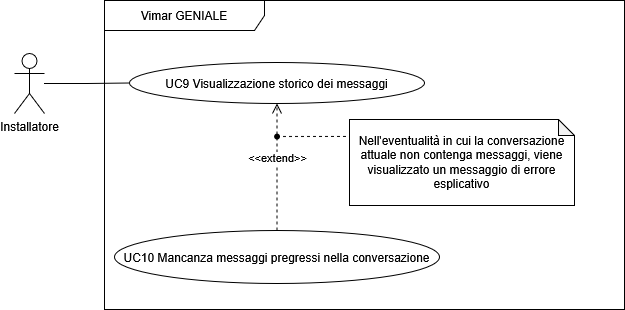
\includegraphics[width=0.8\textwidth]{contents/casi_duso/png/UC9.png}
\caption{UC9 - Visualizzazione storico dei messaggi}
% \label{fig:UC1a}
\end{figure}

\uc{Mancanza messaggi pregressi nella conversazione}{mancanza_messaggi_pregressi}
\begin{itemize}
    \item \textbf{Attori coinvolti}: Installatore;
    \item \textbf{Descrizione}: L’installatore richiede di visualizzare lo storico dei messaggi di una conversazione, ma non ci sono messaggi pregressi nella conversazione attuale;
    \item \textbf{Precondizioni}: 
        \begin{itemize}
            \item L’installatore ha accesso all’interfaccia web del sistema;
            \item L’installatore ha accesso ad una conversazione memorizzabile nel sistema;
            \item La conversazione attuale non contiene messaggi scambiati in precedenza.
        \end{itemize}
    \item \textbf{Postcondizioni}: Il sistema restituisce una risposta che indica l’assenza di messaggi pregressi nella conversazione attuale;
    \item \textbf{Scenario principale}:
    \begin{enumerate}
    \item L’installatore accede all’interfaccia web di Vimar GENIALE;
    \item Accede ad una conversazione presente nel sistema e richiede di visualizzarne uno storico dei messaggi;
    \item Il sistema elabora la richiesta e fornisce una risposta che indica l’assenza di messaggi pregressi nella conversazione attuale;
    \item L’installatore visualizza il messaggio che indica l’assenza di messaggi pregressi.
    \end{enumerate}
\end{itemize}
\begin{figure}[H]
\centering
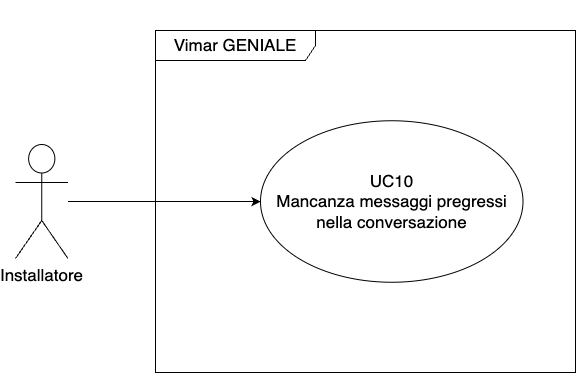
\includegraphics[width=0.8\textwidth]{contents/casi_duso/png/UC10.png}
\caption{UC10 - Mancanza messaggi pregressi nella conversazione}
% \label{fig:UC1a}
\end{figure}


\uc{Fornitura di feedback sulla risposta del sistema ad interrogazione}{fornitura_feedback}
\begin{itemize}
    \item \textbf{Attori coinvolti}: Installatore;
    \item \textbf{Descrizione}: L’installatore, a seguito dell’interrogazione del sistema per ottenere informazioni, desidera fornire un feedback che indichi se la risposta ricevuta sia corretta o meno;
    \item \textbf{Precondizioni}: 
        \begin{itemize}
            \item L’installatore ha accesso all’interfaccia web del sistema;
            \item L’installatore ha accesso ad una conversazione memorizzabile nel sistema;
            \item Il sistema fornisce una risposta ad un’interrogazione da parte dell’installatore.
        \end{itemize}
    \item \textbf{Postcondizioni}: L’installatore, dopo aver esaminato la risposta ricevuta, fornisce un riscontro sulla correttezza di quest’ultima che verrà registrato dal sistema;
    \item \textbf{Scenario principale}:
    \begin{enumerate}
    \item L’installatore accede all’interfaccia web di Vimar GENIALE;
    \item Inserisce una domanda o una parola chiave relativa ad un prodotto specifico;
    \item Il sistema esegue la ricerca nel database dei prodotti e restituisce una risposta che include informazioni dettagliate come schemi, descrizioni e manuali;
    \item L’installatore visualizza le informazioni fornite e, dopo aver verificato la correttezza delle informazioni ricevute, fornisce un feedback sulla risposta al sistema;
    \item Il sistema registra il feedback ricevuto dall’installatore.
    \end{enumerate}
    \item \textbf{Inclusioni} (Le inclusioni hanno senso se verranno svolte azioni aggiuntive rispetto alla sola registrazione del feedback): 
        \begin{itemize}
            \item UC 11.1 - Fornitura di feedback positivo sulla risposta del sistema ad interrogazione
            \item UC 11.2 - Fornitura di feedback negativo sulla risposta del sistema ad interrogazione
        \end{itemize}
\end{itemize}

\subuc{Fornitura di feedback positivo sulla risposta del sistema ad interrogazione}{feedback_positivo}
\begin{itemize}
    \item \textbf{Attori coinvolti}: Installatore;
    \item \textbf{Descrizione}: L’installatore, a seguito dell’interrogazione del sistema per ottenere informazioni, desidera fornire un feedback che indichi che la risposta ricevuta è corretta;
    \item \textbf{Precondizioni}: 
        \begin{itemize}
            \item L’installatore ha accesso all’interfaccia web del sistema;
            \item L’installatore ha accesso ad una conversazione memorizzata nel sistema;
            \item Il sistema fornisce una risposta corretta ad un’interrogazione da parte dell’installatore.
        \end{itemize}
    \item \textbf{Postcondizioni}: L’installatore, dopo aver esaminato la risposta ricevuta, fornisce un riscontro positivo sulla correttezza di quest’ultima che verrà registrato dal sistema;
    \item \textbf{Scenario principale}:
    \begin{enumerate}
    \item L’installatore accede all’interfaccia web di Vimar GENIALE;
    \item Inserisce una domanda o una parola chiave relativa ad un prodotto specifico;
    \item Il sistema esegue la ricerca nel database dei prodotti e restituisce una risposta che include informazioni dettagliate come schemi, descrizioni e manuali;
    \item L’installatore visualizza le informazioni fornite e, dopo aver verificato la correttezza delle informazioni ricevute, fornisce un feedback positivo sulla risposta al sistema;
    \item Il sistema registra il feedback ricevuto dall’installatore.
    \end{enumerate}
\end{itemize}

\subuc{Fornitura di feedback negativo sulla risposta del sistema ad interrogazione}{feedback_negativo}
\begin{itemize}
    \item \textbf{Attori coinvolti}: Installatore;
    \item \textbf{Descrizione}: L’installatore, a seguito dell’interrogazione del sistema per ottenere informazioni, desidera fornire un feedback che indichi che la risposta ricevuta è errata;
    \item \textbf{Precondizioni}: 
        \begin{itemize}
            \item L’installatore ha accesso all’interfaccia web del sistema;
            \item L’installatore ha accesso ad una conversazione memorizzata nel sistema;
            \item Il sistema fornisce una risposta errata ad un’interrogazione da parte dell’installatore.
        \end{itemize}
    \item \textbf{Postcondizioni}: L’installatore, dopo aver esaminato la risposta ricevuta, fornisce un riscontro negativo sulla correttezza di quest’ultima che verrà registrato dal sistema;
    \item \textbf{Scenario principale}:
    \begin{enumerate}
    \item L’installatore accede all’interfaccia web di Vimar GENIALE;
    \item Inserisce una domanda o una parola chiave relativa ad un prodotto specifico;
    \item Il sistema esegue la ricerca nel database dei prodotti e restituisce una risposta che include informazioni dettagliate come schemi, descrizioni e manuali;
    \item L’installatore visualizza le informazioni fornite e, dopo aver verificato la correttezza delle informazioni ricevute, fornisce un feedback negativo sulla risposta al sistema;
    \item Il sistema registra il feedback ricevuto dall’installatore.
    \end{enumerate}
\end{itemize}
\begin{figure}[H]
\centering
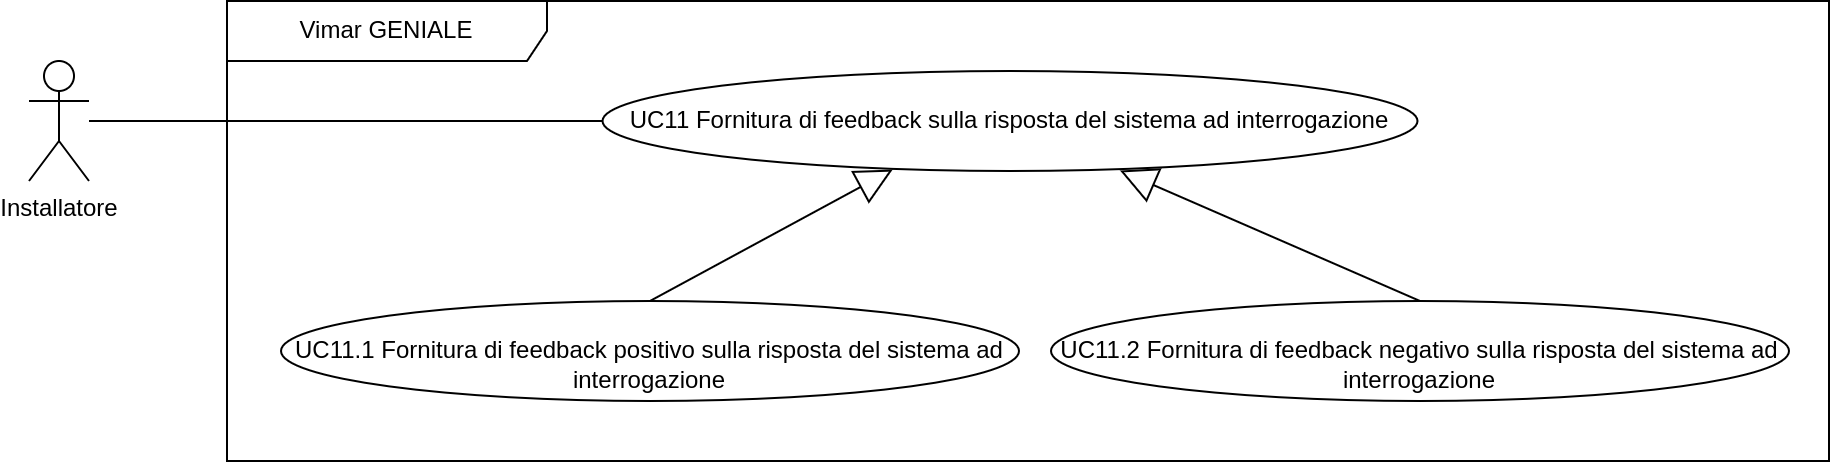
\includegraphics[width=0.8\textwidth]{contents/casi_duso/png/UC11.png}
\caption{UC11 - Fornitura di feedback sulla risposta del sistema ad interrogazione}
% \label{fig:UC1a}
\end{figure}

\uc{Accesso al cruscotto informativo}{accesso_cruscotto}
\begin{itemize}
    \item \textbf{Attori coinvolti}: Amministratore;
    \item \textbf{Descrizione}: Un amministratore desidera accedere al cruscotto informativo per visualizzare una panoramica di informazioni relative all’utilizzo del sistema;
    \item \textbf{Precondizioni}: 
        \begin{itemize}
            \item L’amministratore ha accesso all’interfaccia web del sistema;
            \item L’amministratore è dotato delle credenziali necessarie ad accedere alla dashboard.
        \end{itemize}
    \item \textbf{Postcondizioni}: L’amministratore accede al cruscotto informativo, da cui può visualizzare svariate informazioni riguardanti l’uso del sistema;
    \item \textbf{Scenario principale}:
    \begin{enumerate}
    \item L’amministratore accede all’interfaccia web di Vimar GENIALE;
    \item Inserisce le proprie credenziali;
    \item Il sistema riceve la richiesta di accesso e verifica le credenziali;
    \item L’amministratore ottiene l’accesso alla dashboard.
    \end{enumerate}
    \item \textbf{Estensioni}: UC 13 - Inserimento username o password errati
    \item \textbf{Inclusioni}: 
        \begin{itemize}
            \item UC 12.1 - Inserimento username e password
        \end{itemize}
\end{itemize}


\subuc{Inserimento username e password}{inserimento_username}
\begin{itemize}
    \item \textbf{Attori coinvolti}: Amministratore;
    \item \textbf{Descrizione}: Un amministratore desidera accedere al cruscotto informativo per visualizzare una panoramica di informazioni relative all’utilizzo del sistema, dunque inserisce lo username e la password;
    \item \textbf{Precondizioni}: 
        \begin{itemize}
            \item L’amministratore ha accesso all’interfaccia web del sistema;
            \item L’amministratore è dotato dello username e della password necessarie ad accedere alla dashboard.
        \end{itemize}
    \item \textbf{Postcondizioni}: L’amministratore ha inserito lo username e la password, ovvero le credenziali richieste per l’accesso al cruscotto informativo;
    \item \textbf{Scenario principale}:
    \begin{enumerate}
    \item L’amministratore accede all’interfaccia web di Vimar GENIALE;
    \item Inserisce lo username.
    \item Inserisce la password.
    \end{enumerate}
\end{itemize}


\uc{Inserimento username o password errati}{inserimento_cred_errati}
\begin{itemize}
    \item \textbf{Attori coinvolti}: Amministratore;
    \item \textbf{Descrizione}: Un amministratore desidera accedere al cruscotto informativo per visualizzare una panoramica di informazioni relative all’utilizzo del sistema, ma non riesce ad accedere a causa di un errore nell’inserimento dello username o della password;
    \item \textbf{Precondizioni}: 
        \begin{itemize}
            \item L’amministratore ha accesso all’interfaccia web del sistema;
            \item L’amministratore è dotato delle credenziali necessarie ad accedere alla dashboard;
            \item Lo username o la password non sono corretti.
        \end{itemize}
    \item \textbf{Postcondizioni}: Il sistema restituisce una risposta che indica il motivo per cui si è verificato l’errore;
    \item \textbf{Scenario principale}:
    \begin{enumerate}
    \item L’amministratore accede all’interfaccia web di Vimar GENIALE;
    \item Inserisce le proprie credenziali;
    \item Il sistema elabora la richiesta e fornisce una risposta che spiega l’inserimento errato delle credenziali;
    \item L’amministratore visualizza le informazioni sull’errore che si è verificato.
    \end{enumerate}
\end{itemize}

\begin{figure}[H]
\centering
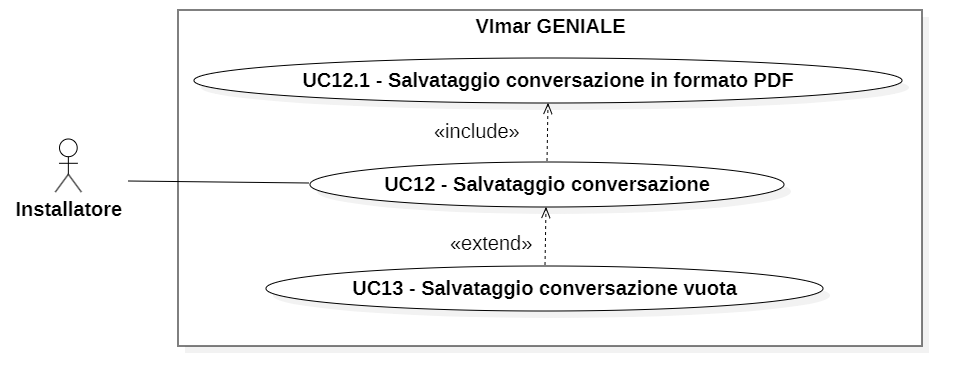
\includegraphics[width=0.8\textwidth]{contents/casi_duso/png/UC12.png}
\caption{UC12, UC12.1 UC13 - Accesso al cruscotto informativo }
% \label{fig:UC1a}
\end{figure}

\uc{Visualizzazione informazioni sulla dashboard}{visualizzazione_info_dashboard}
\begin{itemize}
    \item \textbf{Attori coinvolti}: Amministratore;
    \item \textbf{Descrizione}: Un amministratore desidera visualizzare una panoramica di informazioni relative all’utilizzo del sistema dal cruscotto informativo;
    \item \textbf{Precondizioni}: 
        \begin{itemize}
            \item L’amministratore ha accesso all’interfaccia web del sistema;
            \item L’amministratore è dotato dell’accesso alla dashboard;
        \end{itemize}
    \item \textbf{Postcondizioni}: Il sistema raccoglie le informazioni richieste e le mostra nella dashboard;
    \item \textbf{Scenario principale}:
    \begin{enumerate}
    \item L’amministratore accede all’interfaccia web di Vimar GENIALE;
    \item Inserisce le proprie credenziali;
    \item Il sistema riceve la richiesta di accesso e verifica le credenziali;
    \item L’amministratore ottiene l’accesso alla dashboard;
    \item Il sistema mostra le informazioni richieste sul cruscotto informativo.
    \end{enumerate}
    \item \textbf{Inclusioni}: UC 12 - Accesso al cruscotto informativo
\end{itemize}

\subuc{Visualizzazione numero richieste con conversazione libera sulla dashboard}{visualizzazione_richieste_libere}
\begin{itemize}
    \item \textbf{Attori coinvolti}: Amministratore;
    \item \textbf{Descrizione}: Un amministratore desidera visualizzare dal cruscotto informativo il numero delle richieste effettuate con una conversazione libera;
    \item \textbf{Precondizioni}: 
        \begin{itemize}
            \item L’amministratore ha accesso all’interfaccia web del sistema;
            \item L’amministratore è dotato dell’accesso alla dashboard;
        \end{itemize}
    \item \textbf{Postcondizioni}: Il sistema raccoglie le informazioni relative al numero delle richieste effettuate con una conversazione libera e le mostra nella dashboard;
    \item \textbf{Scenario principale}:
    \begin{enumerate}
    \item L’amministratore accede all’interfaccia web di Vimar GENIALE;
    \item Inserisce le proprie credenziali;
    \item Il sistema riceve la richiesta di accesso e verifica le credenziali;
    \item L’amministratore ottiene l’accesso alla dashboard;
    \item Il sistema mostra le informazioni richieste sul cruscotto informativo.
    \end{enumerate}
    \item \textbf{Inclusioni}: UC 12 - Accesso al cruscotto informativo
    \item \textbf{Generalizzazioni}: UC 14 - Visualizzazione informazioni sulla dashboard
\end{itemize}

\subuc{Visualizzazione numero richieste con conversazione guidata sulla dashboard}{visualizzazione_richieste_guidate}
\begin{itemize}
    \item \textbf{Attori coinvolti}: Amministratore;
    \item \textbf{Descrizione}: Un amministratore desidera visualizzare dal cruscotto informativo il numero delle richieste effettuate con una conversazione guidata;
    \item \textbf{Precondizioni}: 
        \begin{itemize}
            \item L’amministratore ha accesso all’interfaccia web del sistema;
            \item L’amministratore è dotato dell’accesso alla dashboard;
        \end{itemize}
    \item \textbf{Postcondizioni}: Il sistema raccoglie le informazioni relative al numero delle richieste effettuate con una conversazione guidata e le mostra nella dashboard;
    \item \textbf{Scenario principale}:
    \begin{enumerate}
    \item L’amministratore accede all’interfaccia web di Vimar GENIALE;
    \item Inserisce le proprie credenziali;
    \item Il sistema riceve la richiesta di accesso e verifica le credenziali;
    \item L’amministratore ottiene l’accesso alla dashboard;
    \item Il sistema mostra le informazioni richieste sul cruscotto informativo.
    \end{enumerate}
    \item \textbf{Inclusioni}: UC 12 - Accesso al cruscotto informativo
    \item \textbf{Generalizzazioni}: UC 14 - Visualizzazione informazioni sulla dashboard
\end{itemize}

\subuc{Visualizzazione statistiche sul numero di parole usati nelle richieste sulla dashboard}{visualizzazione_statistiche_parole}
\begin{itemize}
    \item \textbf{Attori coinvolti}: Amministratore;
    \item \textbf{Descrizione}: Un amministratore desidera visualizzare dal cruscotto informativo le statistiche sul numero di parole utilizzate;
    \item \textbf{Precondizioni}: 
        \begin{itemize}
            \item L’amministratore ha accesso all’interfaccia web del sistema;
            \item L’amministratore è dotato dell’accesso alla dashboard;
        \end{itemize}
    \item \textbf{Postcondizioni}: Il sistema raccoglie le informazioni relative alle statistiche sul numero di termini utilizzati nelle richieste e le mostra nella dashboard;
    \item \textbf{Scenario principale}:
    \begin{enumerate}
    \item L’amministratore accede all’interfaccia web di Vimar GENIALE;
    \item Inserisce le proprie credenziali;
    \item Il sistema riceve la richiesta di accesso e verifica le credenziali;
    \item L’amministratore ottiene l’accesso alla dashboard;
    \item Il sistema mostra le informazioni richieste sul cruscotto informativo.
    \end{enumerate}
    \item \textbf{Inclusioni}: UC 12 - Accesso al cruscotto informativo
    \item \textbf{Generalizzazioni}: UC 14 - Visualizzazione informazioni sulla dashboard
\end{itemize}

\subuc{Visualizzazione statistiche sulle parole più usate nelle richieste sulla dashboard}{visualizzazione_statistiche_parole_usate}
\begin{itemize}
    \item \textbf{Attori coinvolti}: Amministratore;
    \item \textbf{Descrizione}: Un amministratore desidera visualizzare dal cruscotto informativo le statistiche sulle parole più usate nelle richieste;
    \item \textbf{Precondizioni}: 
        \begin{itemize}
            \item L’amministratore ha accesso all’interfaccia web del sistema;
            \item L’amministratore è dotato dell’accesso alla dashboard;
        \end{itemize}
    \item \textbf{Postcondizioni}: Il sistema raccoglie le informazioni relative alle statistiche sulle parole più usate nelle richieste e le mostra nella dashboard;
    \item \textbf{Scenario principale}:
    \begin{enumerate}
    \item L’amministratore accede all’interfaccia web di Vimar GENIALE;
    \item Inserisce le proprie credenziali;
    \item Il sistema riceve la richiesta di accesso e verifica le credenziali;
    \item L’amministratore ottiene l’accesso alla dashboard;
    \item Il sistema mostra le informazioni richieste sul cruscotto informativo.
    \end{enumerate}
    \item \textbf{Inclusioni}: UC 12 - Accesso al cruscotto informativo
    \item \textbf{Generalizzazioni}: UC 14 - Visualizzazione informazioni sulla dashboard
\end{itemize}

\subuc{Visualizzazione grafico dell’andamento giornaliero dell’utilizzo dell’applicativo sulla dashboard}{visualizzazione_grafico_andamento}
\begin{itemize}
    \item \textbf{Attori coinvolti}: Amministratore;
    \item \textbf{Descrizione}: Un amministratore desidera visualizzare dal cruscotto informativo il grafico dell’andamento giornaliero dell’utilizzo dell’applicativo;
    \item \textbf{Precondizioni}: 
        \begin{itemize}
            \item L’amministratore ha accesso all’interfaccia web del sistema;
            \item L’amministratore è dotato dell’accesso alla dashboard;
        \end{itemize}
    \item \textbf{Postcondizioni}: Il sistema raccoglie le informazioni, crea il grafico dell’andamento giornaliero dell’utilizzo dell’applicativo e lo mostra nella dashboard;
    \item \textbf{Scenario principale}:
    \begin{enumerate}
    \item L’amministratore accede all’interfaccia web di Vimar GENIALE;
    \item Inserisce le proprie credenziali;
    \item Il sistema riceve la richiesta di accesso e verifica le credenziali;
    \item L’amministratore ottiene l’accesso alla dashboard;
    \item Il sistema mostra le informazioni richieste sul cruscotto informativo.
    \end{enumerate}
    \item \textbf{Inclusioni}: UC 12 - Accesso al cruscotto informativo
    \item \textbf{Generalizzazioni}: UC 14 - Visualizzazione informazioni sulla dashboard
\end{itemize}

\subuc{Visualizzazione numero risposte positive dal sistema di feedback sulla dashboard}{visualizzazione_risposte_positive}
\begin{itemize}
    \item \textbf{Attori coinvolti}: Amministratore;
    \item \textbf{Descrizione}: Un amministratore desidera visualizzare dal cruscotto informativo il numero delle risposte positive dal sistema di feedback;
    \item \textbf{Precondizioni}: 
        \begin{itemize}
            \item L’amministratore ha accesso all’interfaccia web del sistema;
            \item L’amministratore è dotato dell’accesso alla dashboard;
        \end{itemize}
    \item \textbf{Postcondizioni}: Il sistema raccoglie le informazioni relative al numero delle risposte positive dal sistema di feedback e le mostra nella dashboard;
    \item \textbf{Scenario principale}:
    \begin{enumerate}
    \item L’amministratore accede all’interfaccia web di Vimar GENIALE;
    \item Inserisce le proprie credenziali;
    \item Il sistema riceve la richiesta di accesso e verifica le credenziali;
    \item L’amministratore ottiene l’accesso alla dashboard;
    \item Il sistema mostra le informazioni richieste sul cruscotto informativo.
    \end{enumerate}
    \item \textbf{Inclusioni}: UC 12 - Accesso al cruscotto informativo
    \item \textbf{Generalizzazioni}: UC 14 - Visualizzazione informazioni sulla dashboard
\end{itemize}

\subuc{Visualizzazione numero risposte negative dal sistema di feedback sulla dashboard}{visualizzazione_risposte_negative}
\begin{itemize}
    \item \textbf{Attori coinvolti}: Amministratore;
    \item \textbf{Descrizione}: Un amministratore desidera visualizzare dal cruscotto informativo il numero delle risposte negative dal sistema di feedback;
    \item \textbf{Precondizioni}: 
        \begin{itemize}
            \item L’amministratore ha accesso all’interfaccia web del sistema;
            \item L’amministratore è dotato dell’accesso alla dashboard;
        \end{itemize}
    \item \textbf{Postcondizioni}: Il sistema raccoglie le informazioni relative al numero delle risposte negative dal sistema di feedback e le mostra nella dashboard;
    \item \textbf{Scenario principale}:
    \begin{enumerate}
    \item L’amministratore accede all’interfaccia web di Vimar GENIALE;
    \item Inserisce le proprie credenziali;
    \item Il sistema riceve la richiesta di accesso e verifica le credenziali;
    \item L’amministratore ottiene l’accesso alla dashboard;
    \item Il sistema mostra le informazioni richieste sul cruscotto informativo.
    \end{enumerate}
    \item \textbf{Inclusioni}: UC 12 - Accesso al cruscotto informativo
    \item \textbf{Generalizzazioni}: UC 14 - Visualizzazione informazioni sulla dashboard
\end{itemize}
\begin{figure}[H]
\centering
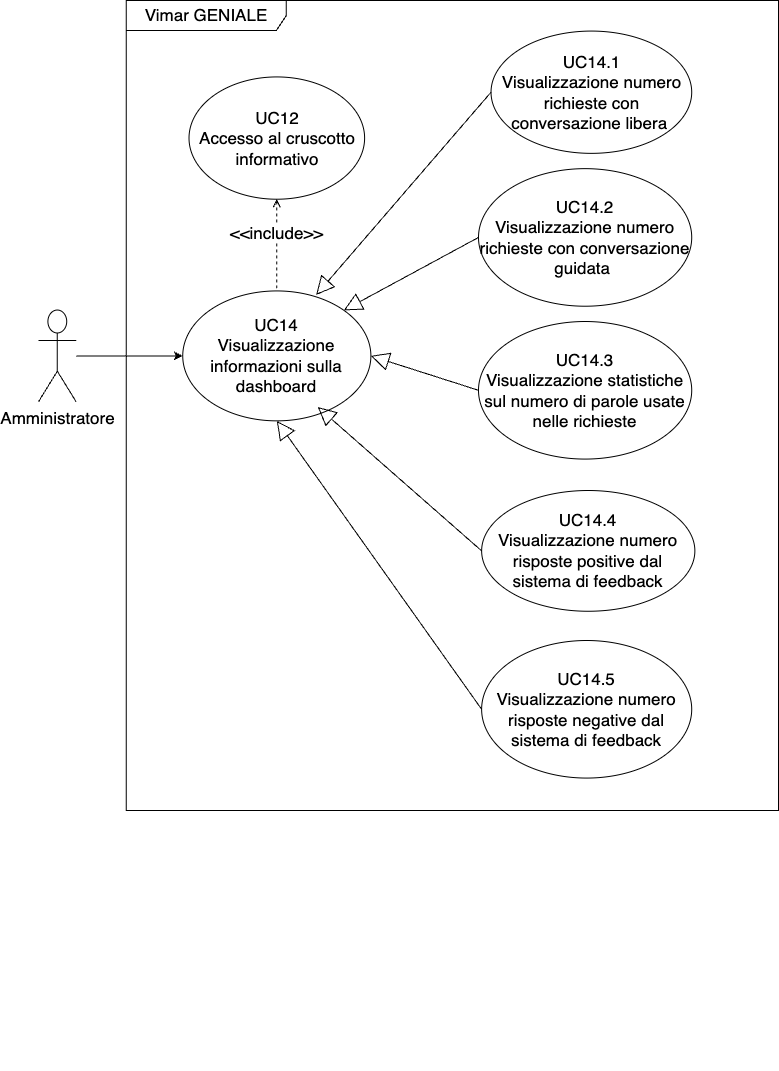
\includegraphics[width=0.8\textwidth]{contents/casi_duso/png/UC14.png}
\caption{UC14 - Visualizzazione informazioni dashboard}
% \label{fig:UC1a}
\end{figure}


\uc{Richiesta di argomento proibito}{argomento_proibito}
\begin{itemize}
    \item \textbf{Attori coinvolti}: Installatore;
    \item \textbf{Descrizione}: L’installatore richiede argomenti proibiti al sistema (e.g. politica, finanza, pornografia, ...);
    \item \textbf{Precondizioni}: 
        \begin{itemize}
            \item L’installatore ha accesso all’interfaccia web del sistema;
            \item L’installatore ha accesso ad una conversazione memorizzabile nel sistema;
            \item La domanda posta non riguarda argomenti proibiti.
        \end{itemize}
    \item \textbf{Postcondizioni}: Il sistema restituisce una risposta che indica il motivo per cui si è verificato l’errore;
    \item \textbf{Scenario principale}:
    \begin{enumerate}
    \item L’installatore accede all’interfaccia web di Vimar GENIALE;
    \item Inserisce una domanda inconsistente, che non ha a che vedere con prodotti VIMAR;
    \item Il sistema elabora la richiesta e fornisce una risposta che spiega la causa dell'errore riscontrato;
    \item L’installatore visualizza le informazioni sull’errore che si è verificato;
    \end{enumerate}
     \item \textbf{Generalizzazioni}: UC 8 - Assenza di informazioni sul prodotto ricercato.
\end{itemize}
\begin{figure}[H]
\centering
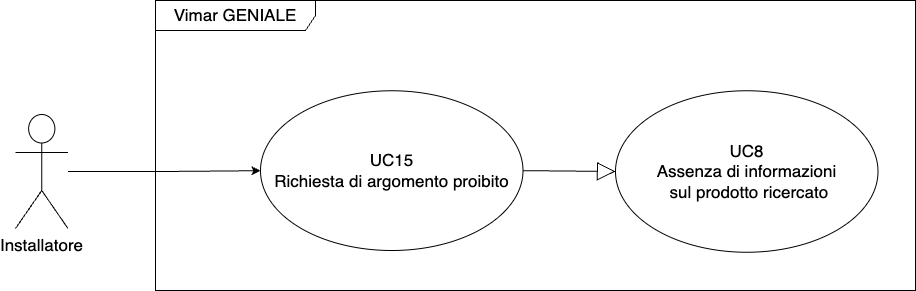
\includegraphics[width=0.8\textwidth]{contents/casi_duso/png/UC15.png}
\caption{UC15 - Richiesta di argomento proibito}
% \label{fig:UC1a}
\end{figure}